
	\subsection{Circuito sin etapa de potencia}
		A continuación se exponen las mediciones realizadas los días \texttt{4/12/2018} y \texttt{5/12/2018} donde se valida el funcionamiento de la primer y segunda etapa del circuito. Para realizar las mismas, se desconectan las conexiones del multiplicador de $V_{BE}$ con los transistores de salida; también se conecta la realimentación global a la salida del VAS dado que el mismo provee la misma tensión que la salida del circuito completo. Sin embargo para emular la conexión de la tercer etapa, se conecta una resistencia de valor comercial \SI{39}{\kilo\ohm} que es aproximadamente igual a la carga que presenta la reflexión de $R_L$ (con valor teórico de \SI{36}{\kilo\ohm}).\\
		\Juan{Poner bancos de medición}
		\indent Con dichas consideraciones se procede a realizar las mediciones.
		\graficarEPS{0.6}{banco_med}{Diagrama del circuito para mediciones sin etapa de potencia.}{fig:banco_med}

		\subsubsection{Polarización}
		
		Las mediciones de polarización se realizaron con el multímetro \emph{UT30D} cortocircuitando la entrada y se exponen en la Figura \ref{fig:51218_pol}. Cabe destacar que las mediciones en color rojo corresponden a tensiones con respecto a masa y aquellas en color azul, diferencia de potencial.
		\begin{figure}[h!]
			\centering
			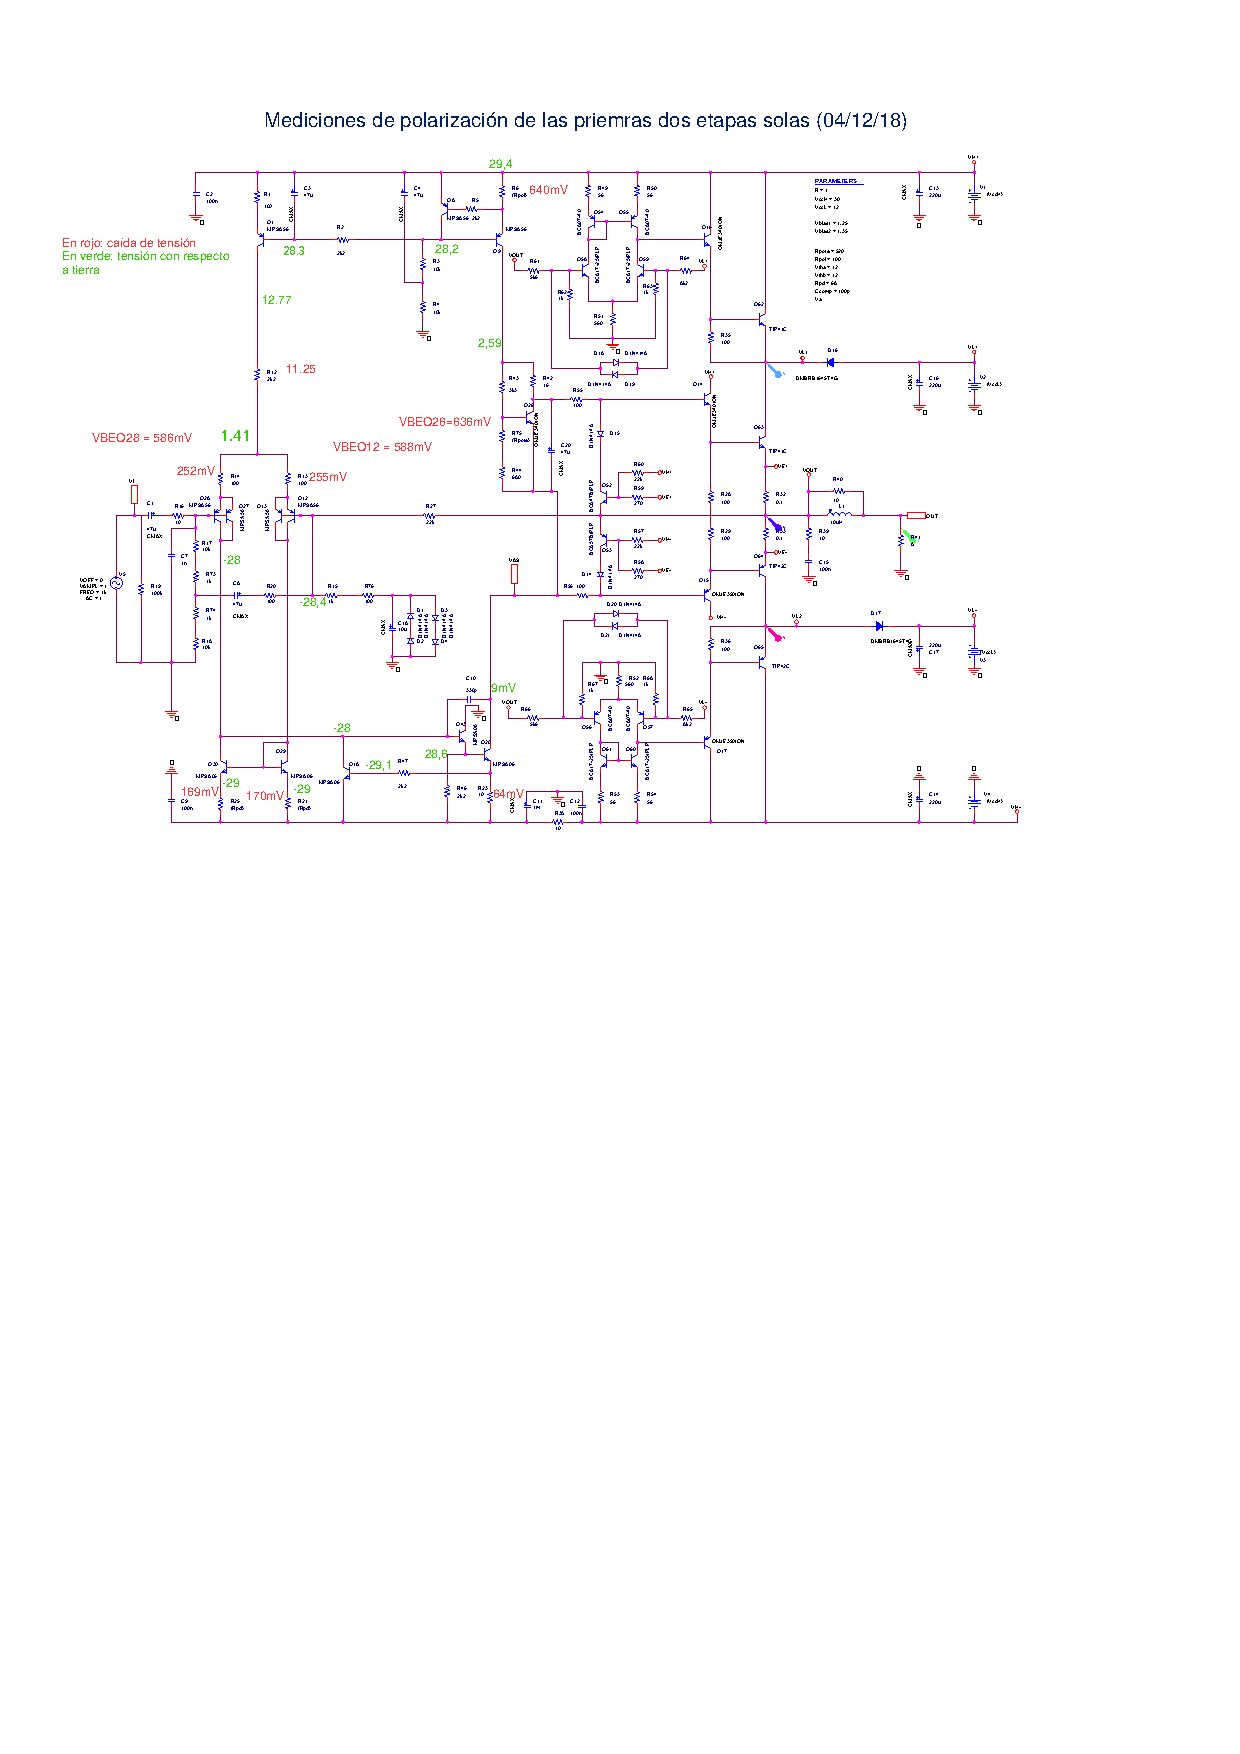
\includegraphics[width=0.8\textwidth, trim = 2cm 14cm 4cm 1cm]{./Mediciones/1_mediciones.pdf}
			\caption{Mediciones de polarización del día \texttt{4/12/2018}.}
			\label{fig:51218_pol}
		\end{figure}

		\subsubsection{Impedancia de entrada}
			
		\begin{figure}[ H]
			\centering
			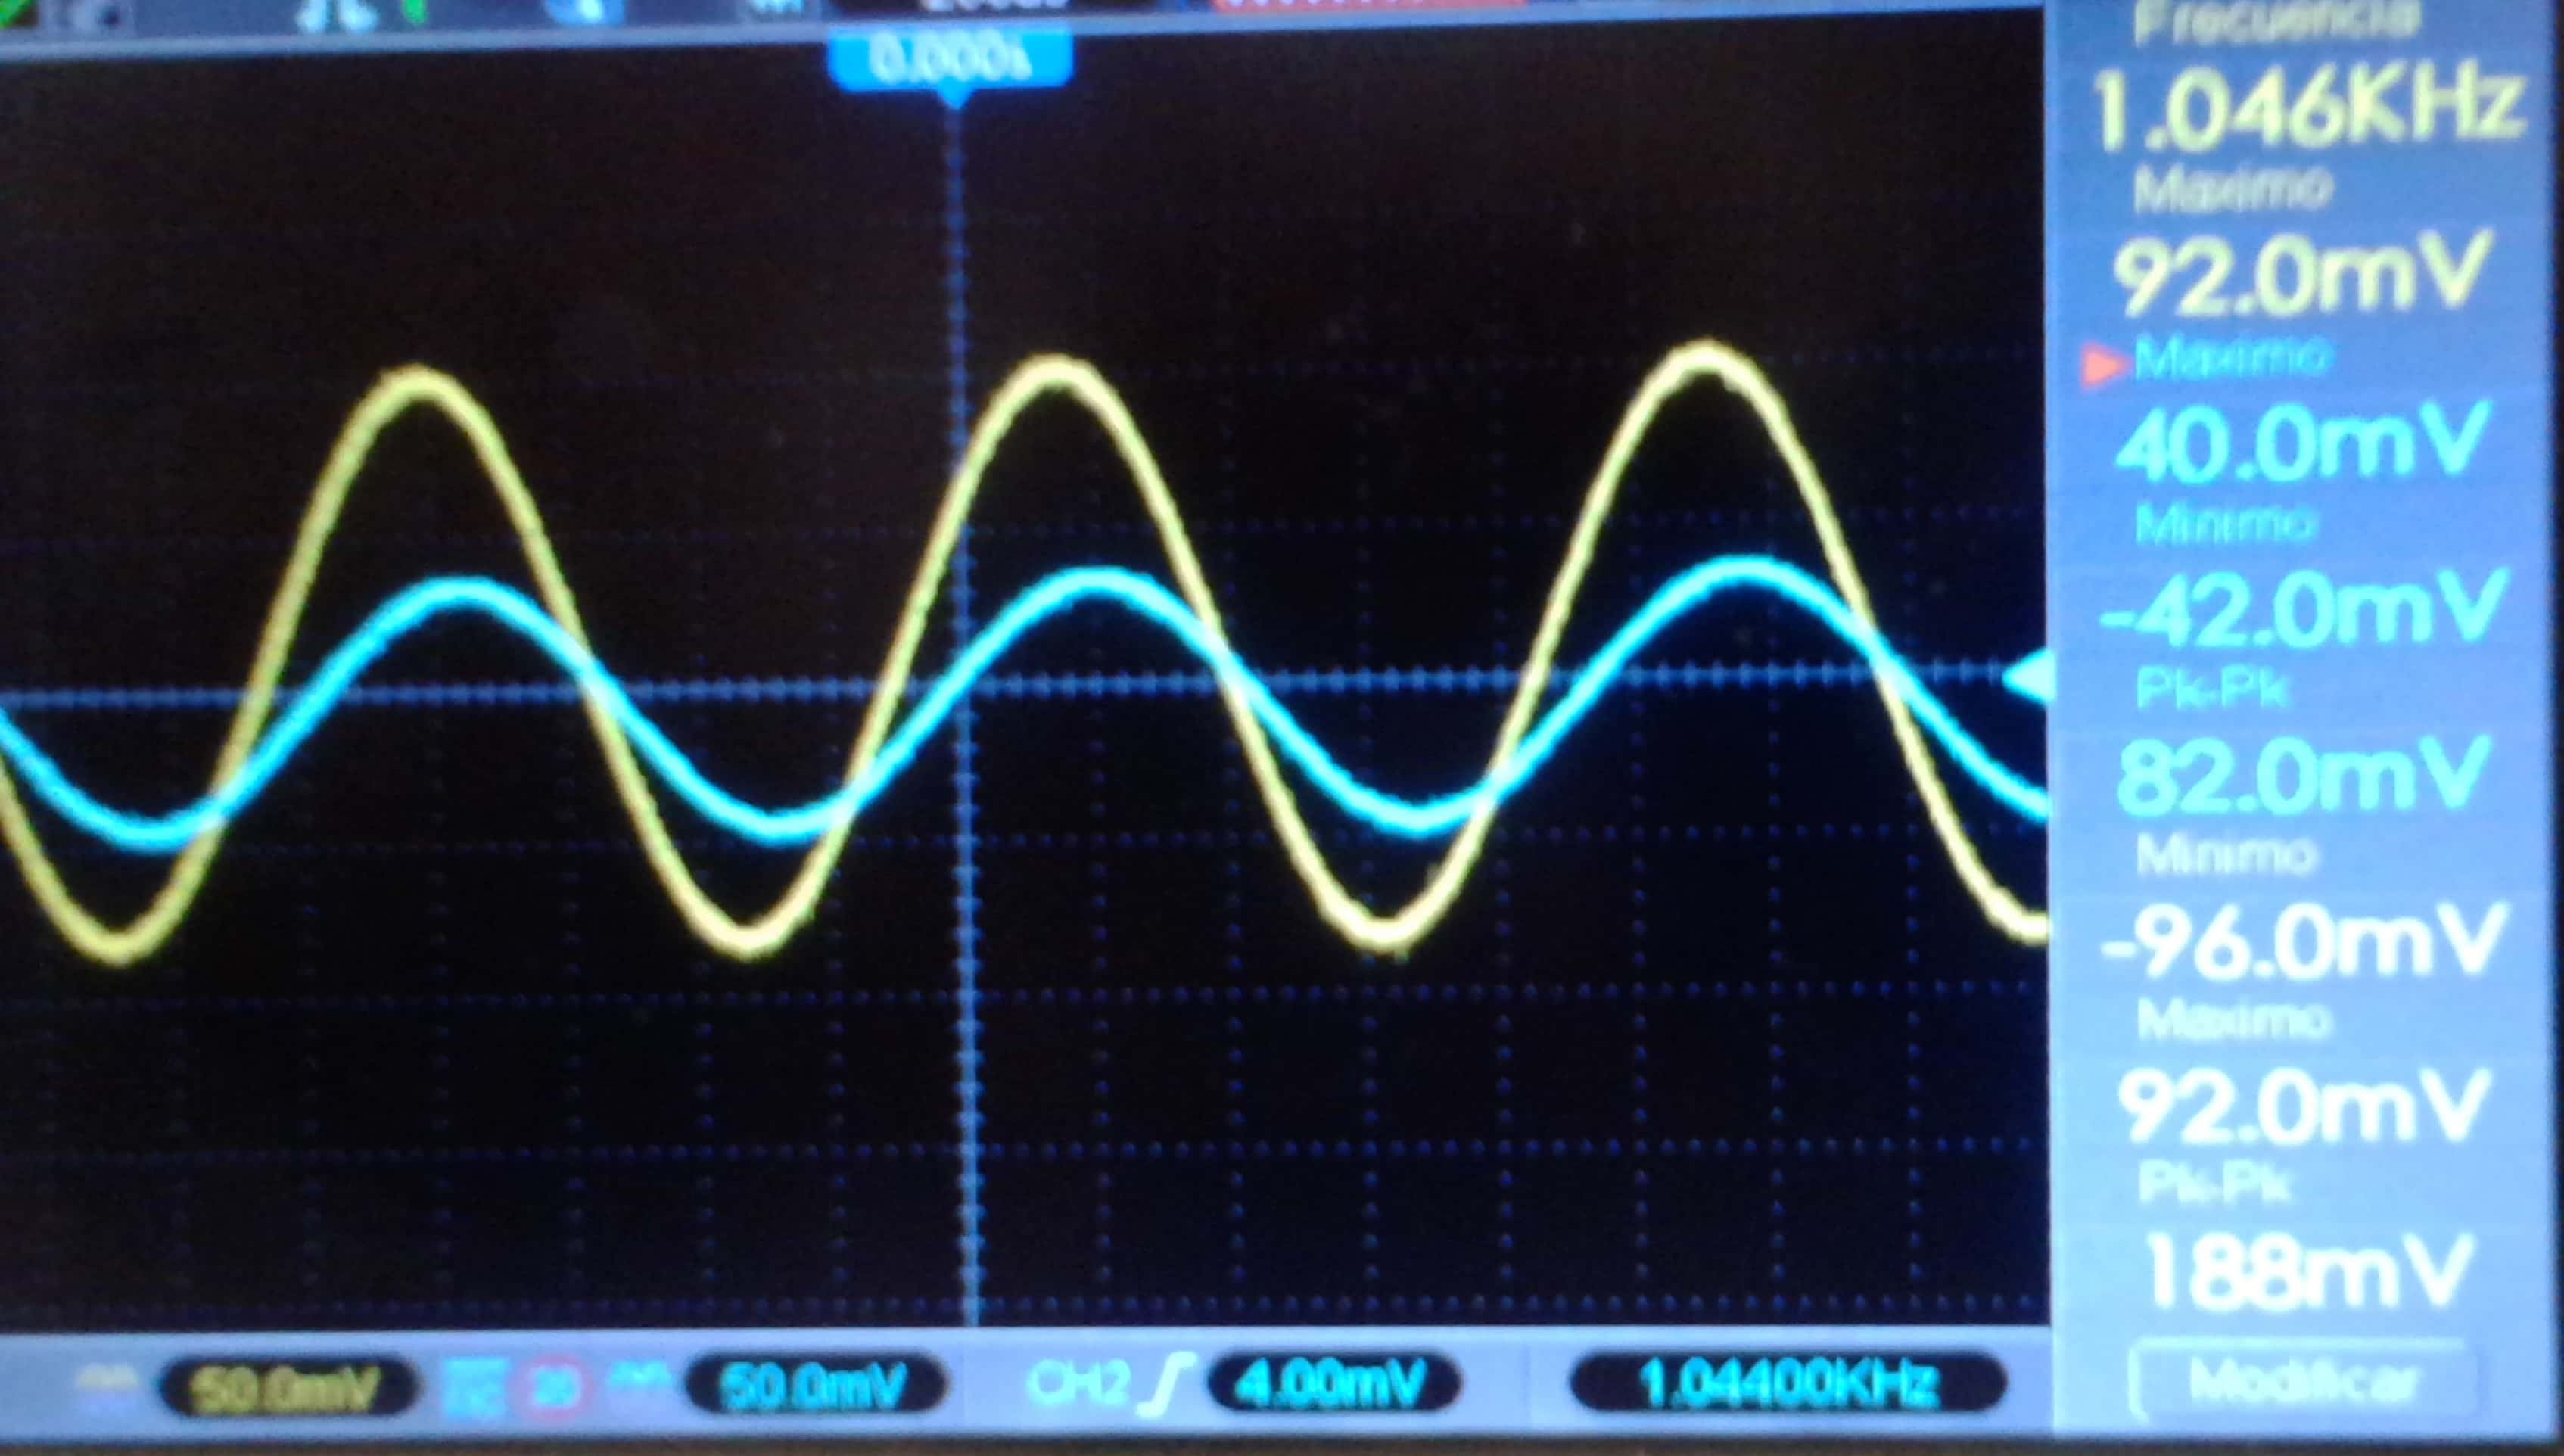
\includegraphics[width=0.8\textwidth]{./Mediciones/Rin_1k.jpg}
			\caption{Medición de las tensiones de generador de prueba y el nodo de entrada.}
			\label{fig:rin_med}
		\end{figure}

		\begin{figure}[ H]
			\centering
			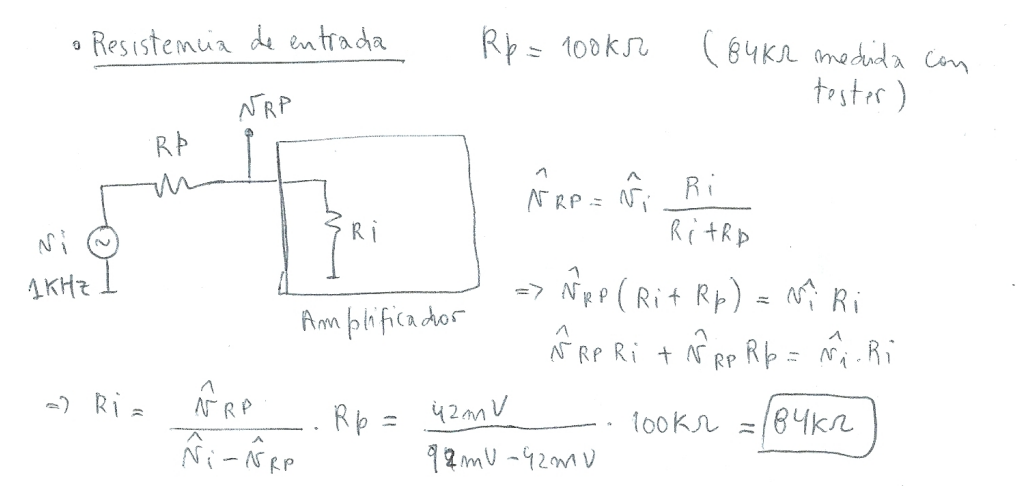
\includegraphics[width=1.0\textwidth]{./Mediciones/Rin_1k_calculo.png}
			\caption{Análisis detallado de la medición de $R_{in}$.}
			\label{fig:analisis_rin_med}
		\end{figure}

		Para la medición de resistencia de entrada, se inyecta una señal conocida al circuito con resistencia serie lo más similar posible a la resistencia de entrada propia del amplificador. La tensión medida está relacionada con el divisor resistivo generado entre $R_{p}$ y $R_{in}$ de forma tal que se puede hallar indirectamente dicha resistencia. La medición se expone en la Figura \ref{fig:rin_med} y en la Figura \ref{fig:analisis_rin_med} se realiza la explicación y cálculo de dicha resistencia resultando $\boxed{R_{in}=\SI{84}{\kilo\ohm}}$.\\

		Del mismo modo se realizó la medición de $R_{in}$ para frecuencia de \SI{10}{\kHz} resultando en:
		\begin{equation*}
			R_{in}(@\SI{10}{\kHz})  = \frac{\SI{13.2}{\mV}}{\SI{94}{\mV} - \SI{13.2}{\mV}} \, \SI{100}{\kilo\ohm} = \boxed{\SI{16.3}{\kilo\ohm}}
		\end{equation*}
		\subsubsection{Ancho de banda de potencia}
		\Juan{No tendría que ser $SR = \omega \cdot \hat{V} = \SI{96.5}{\kHz}$??}

	\graficarEPS{1.0}{Mediciones/graf_BW_pot}{Respuesta en frecuencia para tensiones de entrada $V_{pp} = \SI{1.1}{\V}$.}{fig:pot_BW_med}
		
		\begin{equation*}
			\boxed{f_H \approx \SI{130}{\kHz}}
		\end{equation*}

		\subsubsection{Respuesta al escalón}
		\begin{figure}[h!]
			\centering
			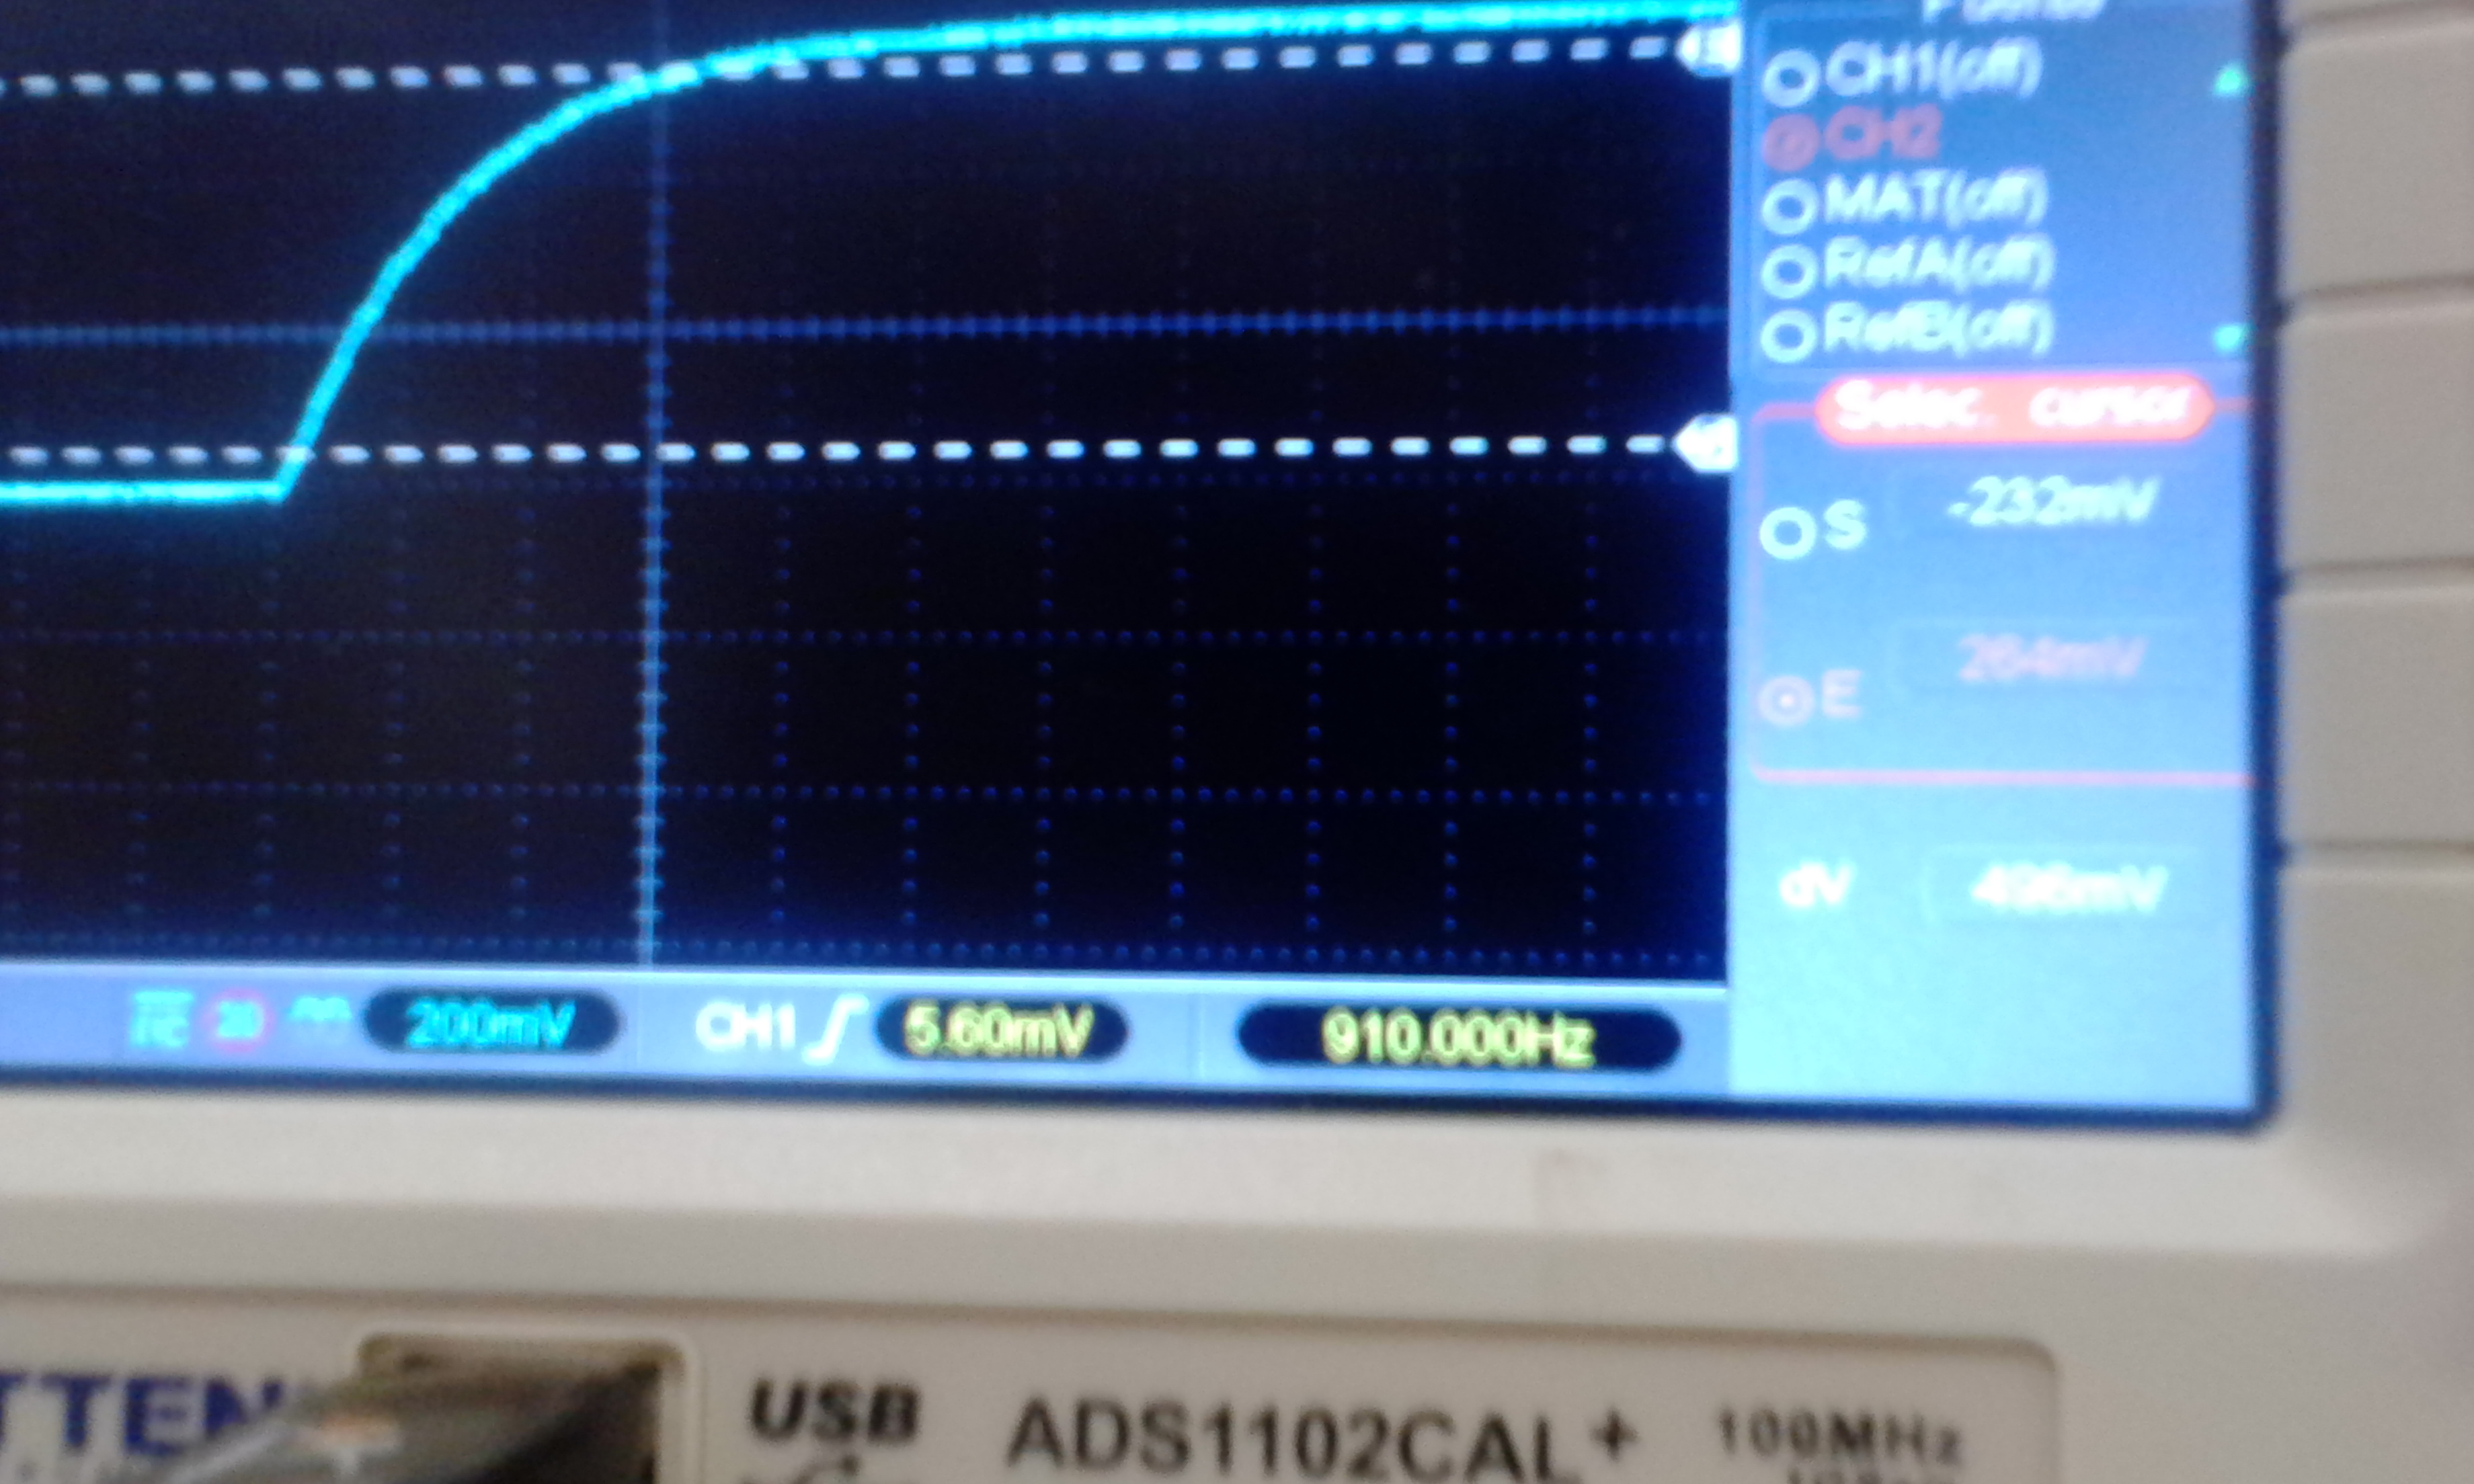
\includegraphics[width=0.8\textwidth]{./Mediciones/BW.jpg}
			\caption{Respuesta al escalón en pequeña señal.}
			\label{fig:escalon_ss}
		\end{figure}

		\begin{figure}[h!]
			\centering
			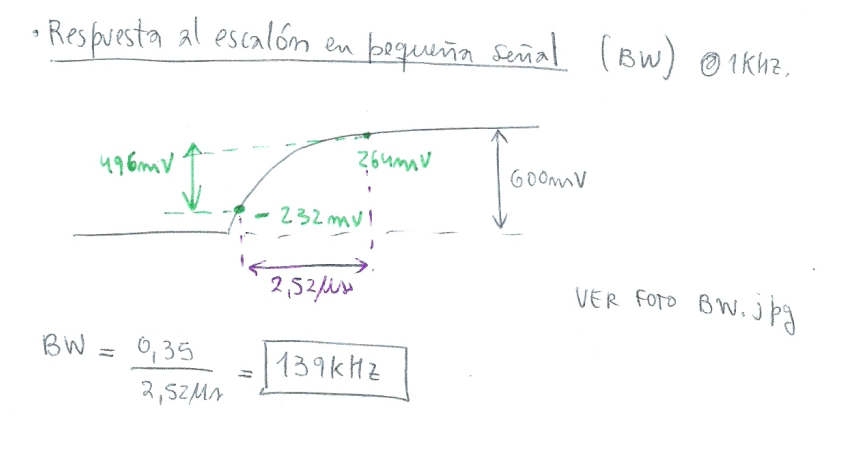
\includegraphics[width=1.0\textwidth]{./Mediciones/BW_calculo.png}
			\caption{Análisis detallado de la medición de respuesta al escalón en señal.}
			\label{fig:analisis_escalon_ss}
		\end{figure}

		Se conecta un generador a la entrada con un escalón de \SI{1}{\kHz} según el banco de medición de la Figura \ref{fig:banco_bw}. La medición se expone en la Figura \ref{fig:escalon_ss} y el análisis del mismo se detalla en la Figura \ref{fig:analisis_escalon_ss} resultando en
		\begin{equation*}
			\boxed{BW = \SI{139}{\kHz}}
		\end{equation*}

		\subsubsection{\emph{Slew Rate}}
		Se realiza una medición similar a la anterior, salvo que en este caso la entrada es un escalón que va de \SI{-.6}{\V} a \SI{.6}{\V}. Así a partir de la medición de la Figura \ref{fig:sr_med} como se detallan los valores en la Figura \ref{fig:analisis_sr_med} se obtiene un \emph{Slew Rate} similar al simulado de $\boxed{SR = \SI{8}{\V\per\micro\second}}$.

		\begin{figure}[h!]
			\centering
			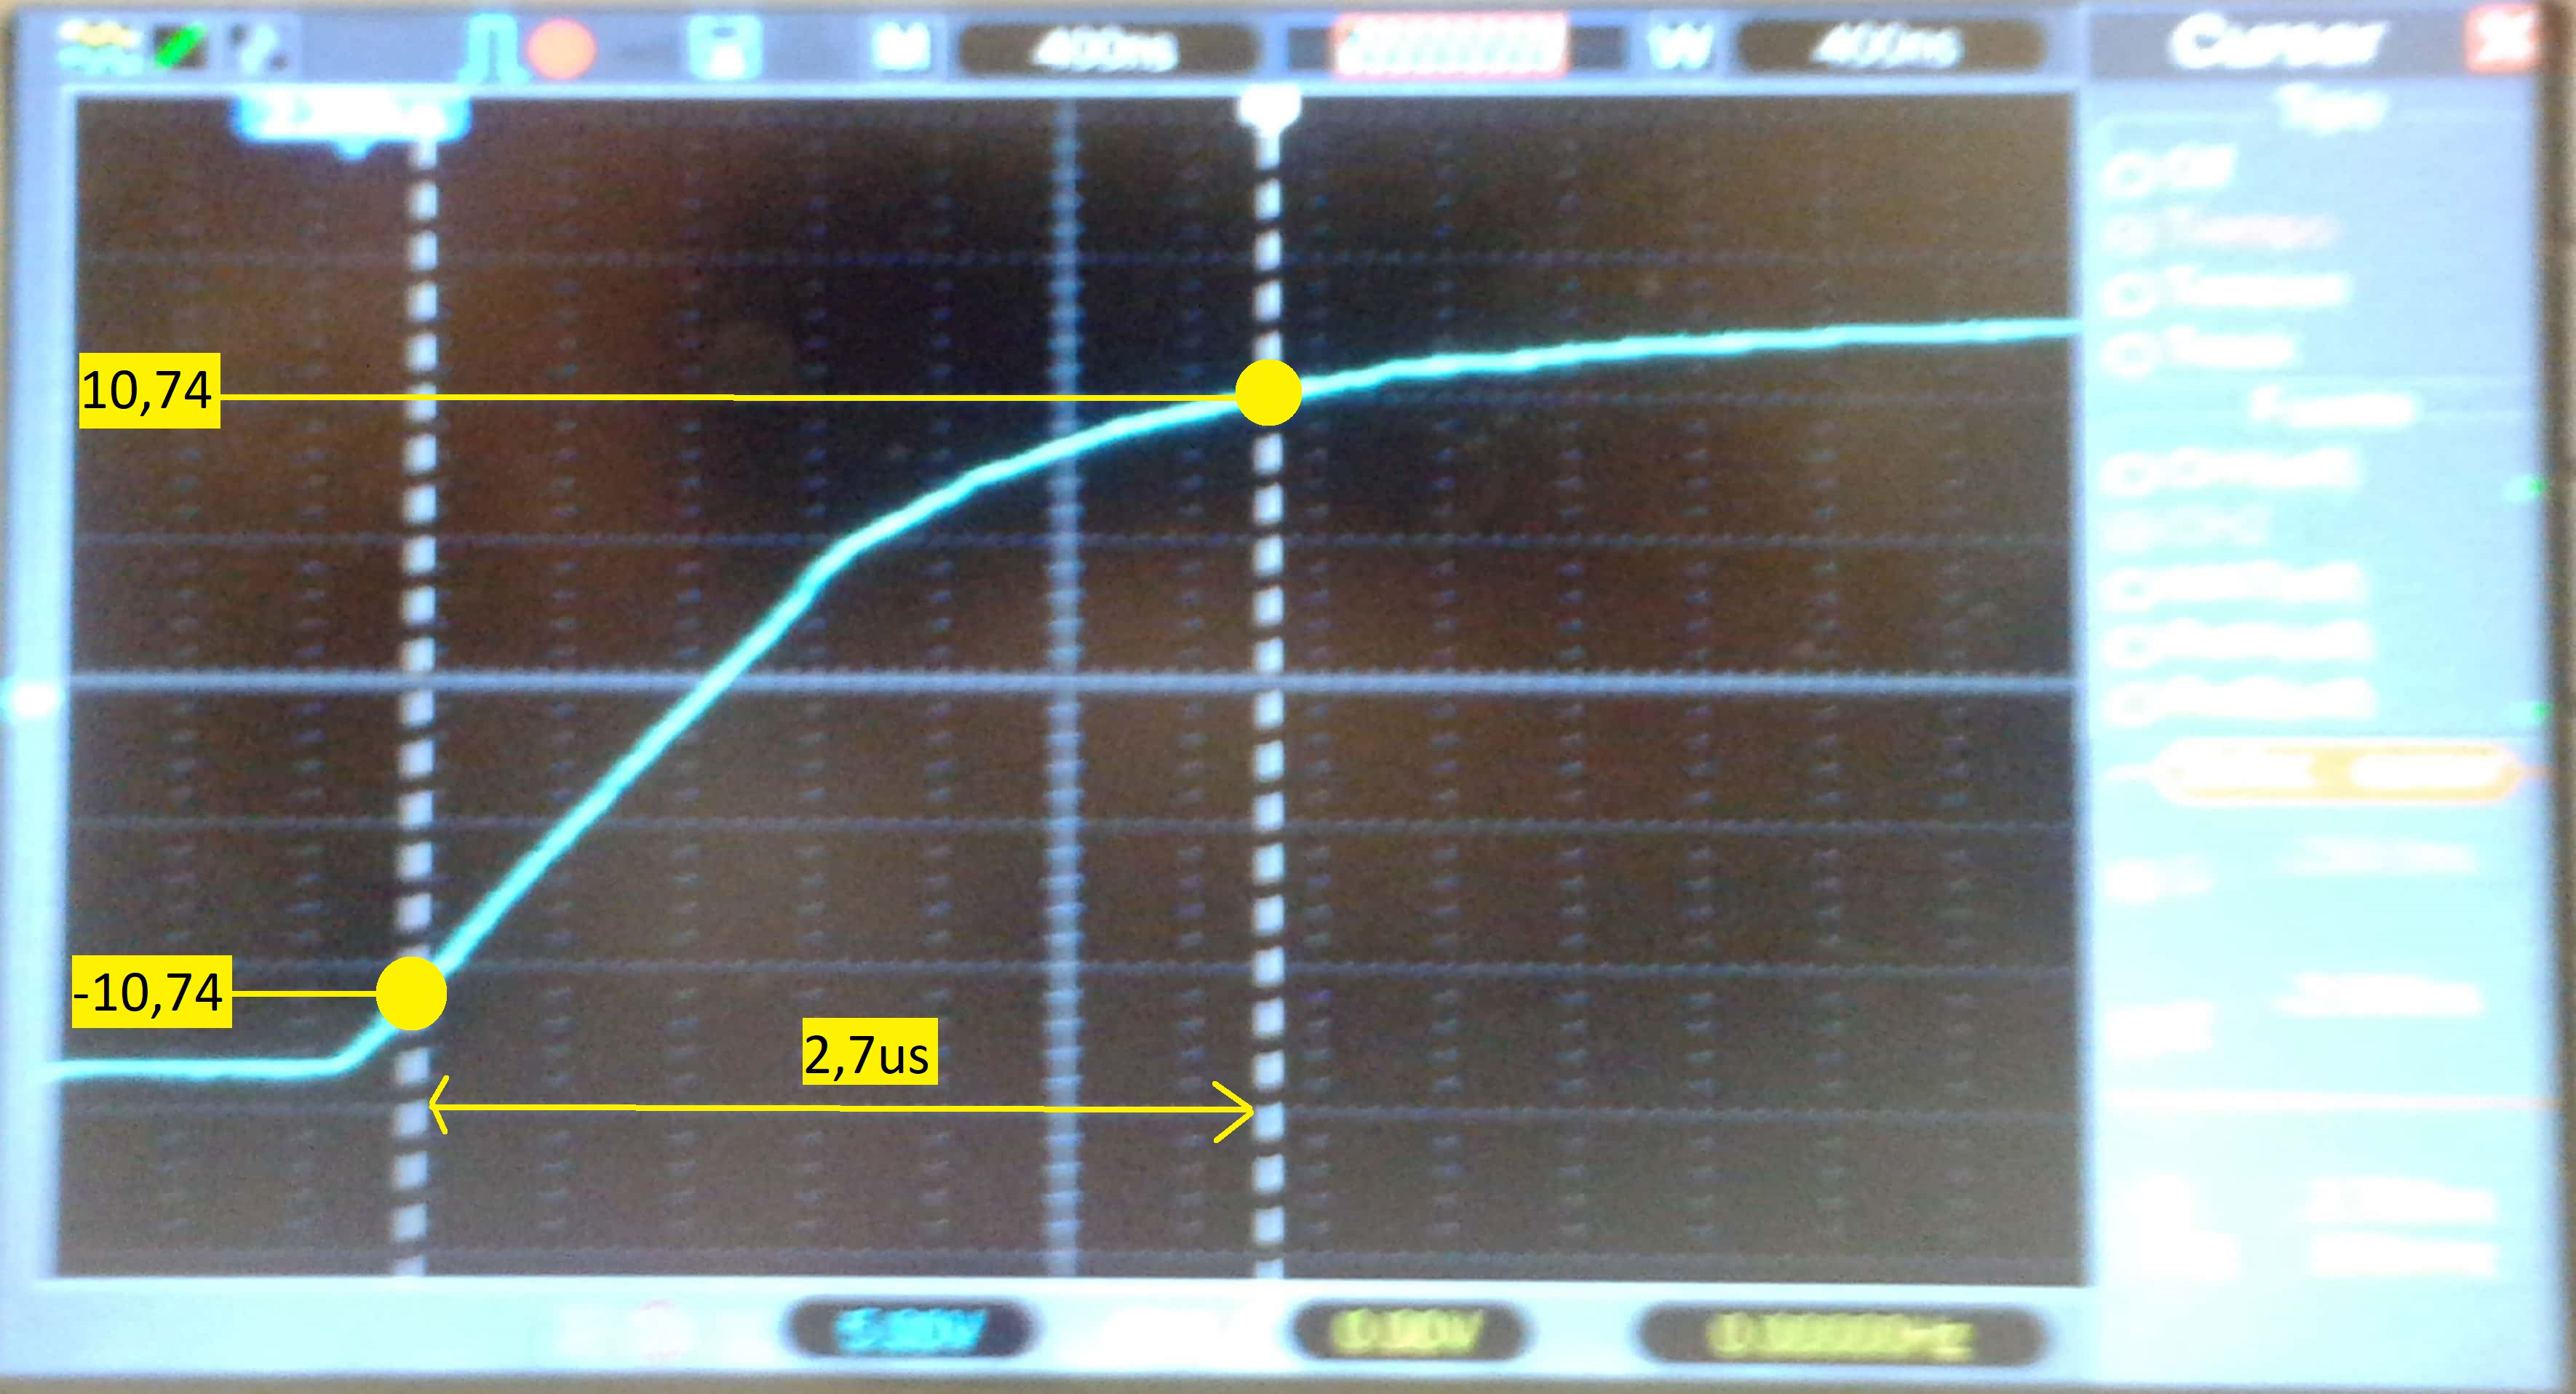
\includegraphics[width=0.8\textwidth]{./Mediciones/SR2.jpg}
			\caption{Respuesta al escalón en gran señal para hallar el \emph{Slew Rate}.}
			\label{fig:sr_med}
		\end{figure}

		\begin{figure}[h!]
			\centering
			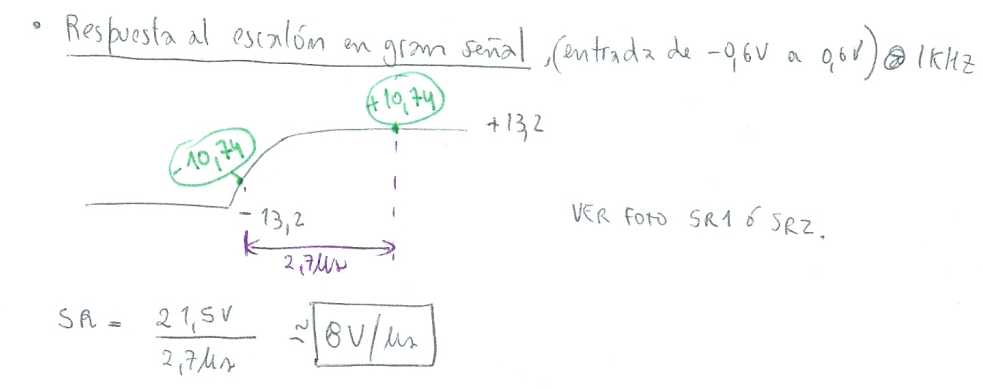
\includegraphics[width=1.0\textwidth]{./Mediciones/SR_calculo.png}
			\caption{Análisis detallado de la medición del \emph{Slew Rate}.}
			\label{fig:analisis_sr_med}
		\end{figure}

		\subsubsection{Variación de la Fuente de Alimentación}
		
		\graficarPNG{0.4}{./Mediciones/Variacion_fuente}{Mediciones de las caídas de potencial para 2 juegos de tensiones de alimentación.}{fig:var_fuente_med}
		En este caso se alimentó el circuito con $V_{CCH+}$ y $V_{CCH-}$ pero se supone que dichas fuentes no son muy buenas. Por tanto se midieron las caídas de potencial sobre las resistencias con los valores de alimentación común y con alimentaciones menores al 10\%. Los resultados y mediciones se exponen en la Figura \ref{fig:var_fuente_med} mostrando errores menores al \num{1.8}\%.


		\subsubsection{Distorsión armónica}
			Se realizó un análsis de \emph{FFT} del circuito ingresando con una señal de \SI{1}{\kHz}, pero no se pueden sacar conclusiones de la medición de la Figura \ref{fig:fft_med} porque el piso de ruido es muy alto y no se puede ver el efecto de los harmónicos. Para ello habría que utilizar un \emph{software} que permita ingresar señales particulares y ver el comportamiento en frecuencia del circuito ante esos estímulos.

		\graficarPNG{0.1}{./Mediciones/FFT}{Análisis del circuito por Fourier.}{fig:fft_med}

		\subsubsection{Máxima excursión de salida}
			
		Se introdujo una señal de amplitud tal que la salida no recorte. Dicha señal corresponde a una de amplitud pico a pico \SI{1.1}{\V}. A la salida se obtiene $V_{pp} = \SI{32.4}{\V}$.

		\HgraficarPNG{0.1}{./Mediciones/Maxima_excursion}{Medición de máxima excursión de salida sin recorte.}{fig:excursion_med}


%		\subsubsection{Compensación}
%
%		\subsubsection{Respuesta en frecuencia}
%
%		\subsubsection{Impedancia de salida}
%
%		\subsubsection{Margen de fase}
%
%		\subsubsection{Distorsión por intermodulación}
%		
%		\subsubsection{Rechazo de Ruido de la Fuente de Alimentación}
%
%		\subsubsection{Máxima eficiencia del amplificador}
%
%		\subsubsection{Comportamiento térmico}
